\section{結果のクイック描画:SNO} \label{sec:quicklook}
%####################################################################################

本節では、\sno の使用方法を説明する。
プログラム\sno は、プロセス毎に分割された{\netcdf}ファイル(\verb|history.**.nc|
\footnote{「gpview」がインストールされている場合には、「gpview」でも作図することができる。
このツールは historyデータを変換することなく直接作図することができるため、
素早く結果を確認した場合には適している。
}
)
を{\grads}が読み込み可能な単一の{\netcdf}ファイルに結合することもできる。
この変換した{\netcdf}データを使って、シミュレーションの結果を確認する。


\subsubsection{{\grads}読み込み可能な{\netcdf}に変換}
%-----------------------------------------------------------------------------------
プロセスごとに分割された{\netcdf}形式のヒストリファイルから{\grads}が読み込み可能な{\netcdf}ファイルに変換するために、\sno を使用する。
ここでは最低限の手順のみを説明することにする。
詳細な使用方法は\ref{sec:sno}節を参照されたい。

まず、\sno ディレクトリに移動する。
\begin{verbatim}
 $ cd ${Tutorial_DIR}/real/experiment/sno
 $ ls
    Makefile
    sno -> ../../../../../../bin/sno
    sno.hgridope.d01.conf
    sno.vgridope.d01.conf
\end{verbatim}
このディレクリの中には設定ファイルとバイナリファイルがある。
バイナリファイルは、\ref{sec:compile_sno}節でコンパイルした実行ファイルにリンクされている。
ここでは例として、全変数を{\grads}に読み込み可能な{\netcdf}ファイルへ変換する手順を示す。

\sno を実行する時のプロセス数は、シミュレーションの実行時に用いたプロセス数の約数である必要がある。
ここでは、4プロセスを使用する。
\sno は鉛直軸方向と水平軸方向の変換を同時に変換できないために、以下のように別々に実行する。
\begin{verbatim}
 $ mpirun -n 4 ./sno sno.vgridope.d01.conf
 $ mpirun -n 4 ./sno sno.hgridope.d01.conf
\end{verbatim}
エラーメッセージがなく、下記のメッセージだけが標準出力へ表示されていれば、変換は正常に完了している。
\msgbox{
\verb|*** End   SCALE-NetCDF Operator| \\
}

成功すれば、下記のファイルが作成される。

\begin{verbatim}
  merged-h_history_d01.pe000000.nc
\end{verbatim}




\subsubsection{計算結果の確認}
%-----------------------------------------------------------------------------------

%\verb|${Tutorial_DIR}/real/data|ディレクトリに用意してあるので、
%サンプルとして利用してほしい。\footnote{今後、緯度経度座標で描画するためのctlファイルを出力できるようにする予定。}
%\begin{verbatim}
% $ cp ../../data/*_lcc.ctl ./
% $ ls
%    MSLP_d01z-2d_lcc.ctl
%    PREC_d01z-2d_lcc.ctl
%    U_d01z-3d_lcc.ctl
%    V_d01z-3d_lcc.ctl
%\end{verbatim}

\grads スクリプト\verb|checkfig_real.gs|を用いて、計算結果を確認する。
\begin{verbatim}
 $ cp ../../data/checkfig_real.gs ./
 $ grads -blc checkfig_real.gs
\end{verbatim}
変換が正常に終了すれば、下記のファイルが作成される。
なお、\grads のバージョンによって文法が異なるので、警告が出る場合はスクリプトを適宜変更されたい。
\begin{verbatim}
  real_mslp.png
  real_prec.png
  real_wind.png
\end{verbatim}
計算が成功していれば、図\ref{fig:real_mslp}, \ref{fig:real_prec}, \ref{fig:real_wind}と同じ図が得られる。


\begin{figure}[h]
\begin{center}
  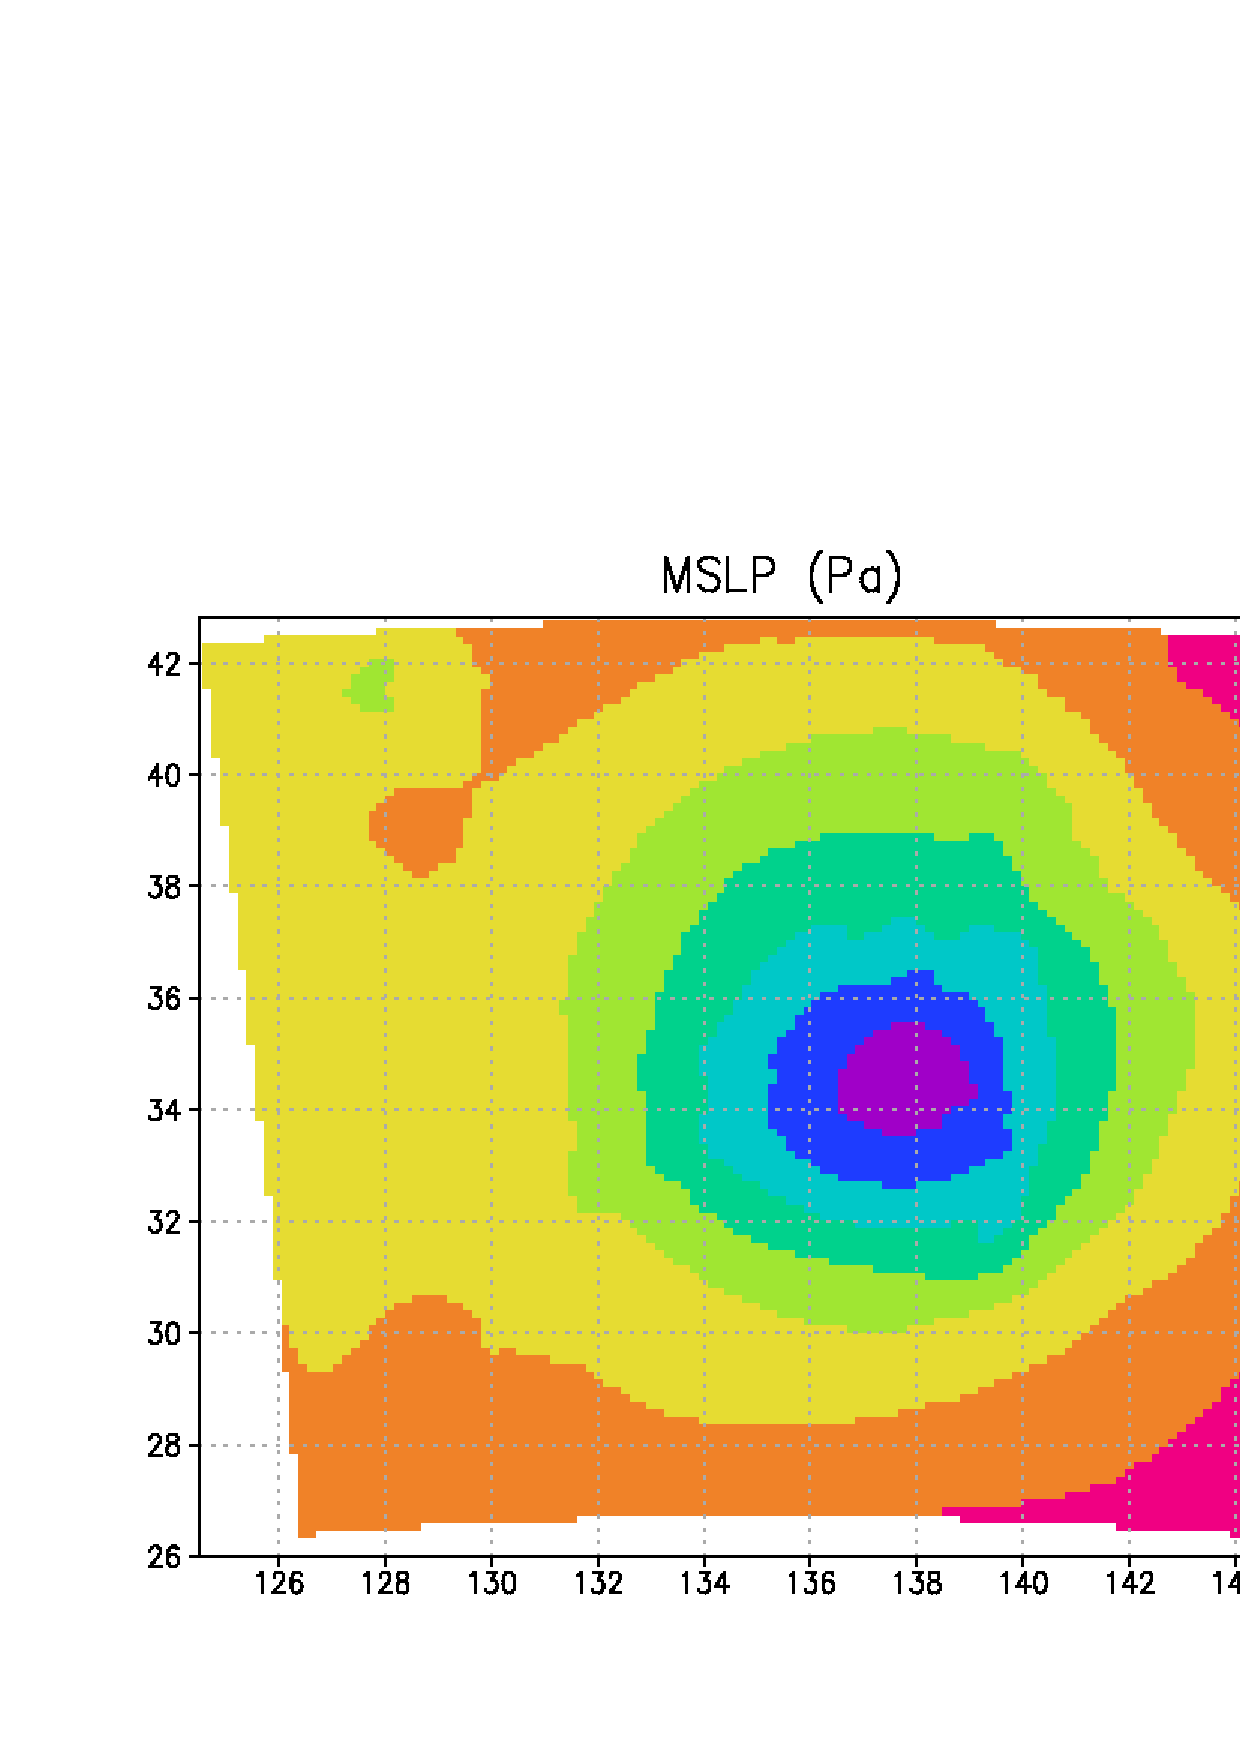
\includegraphics[width=0.55\hsize]{./../../figure/real_mslp.pdf}\\
  \caption{計算開始から6時間後の海面更正気圧}
  \label{fig:real_mslp}
\end{center}
\begin{center}
  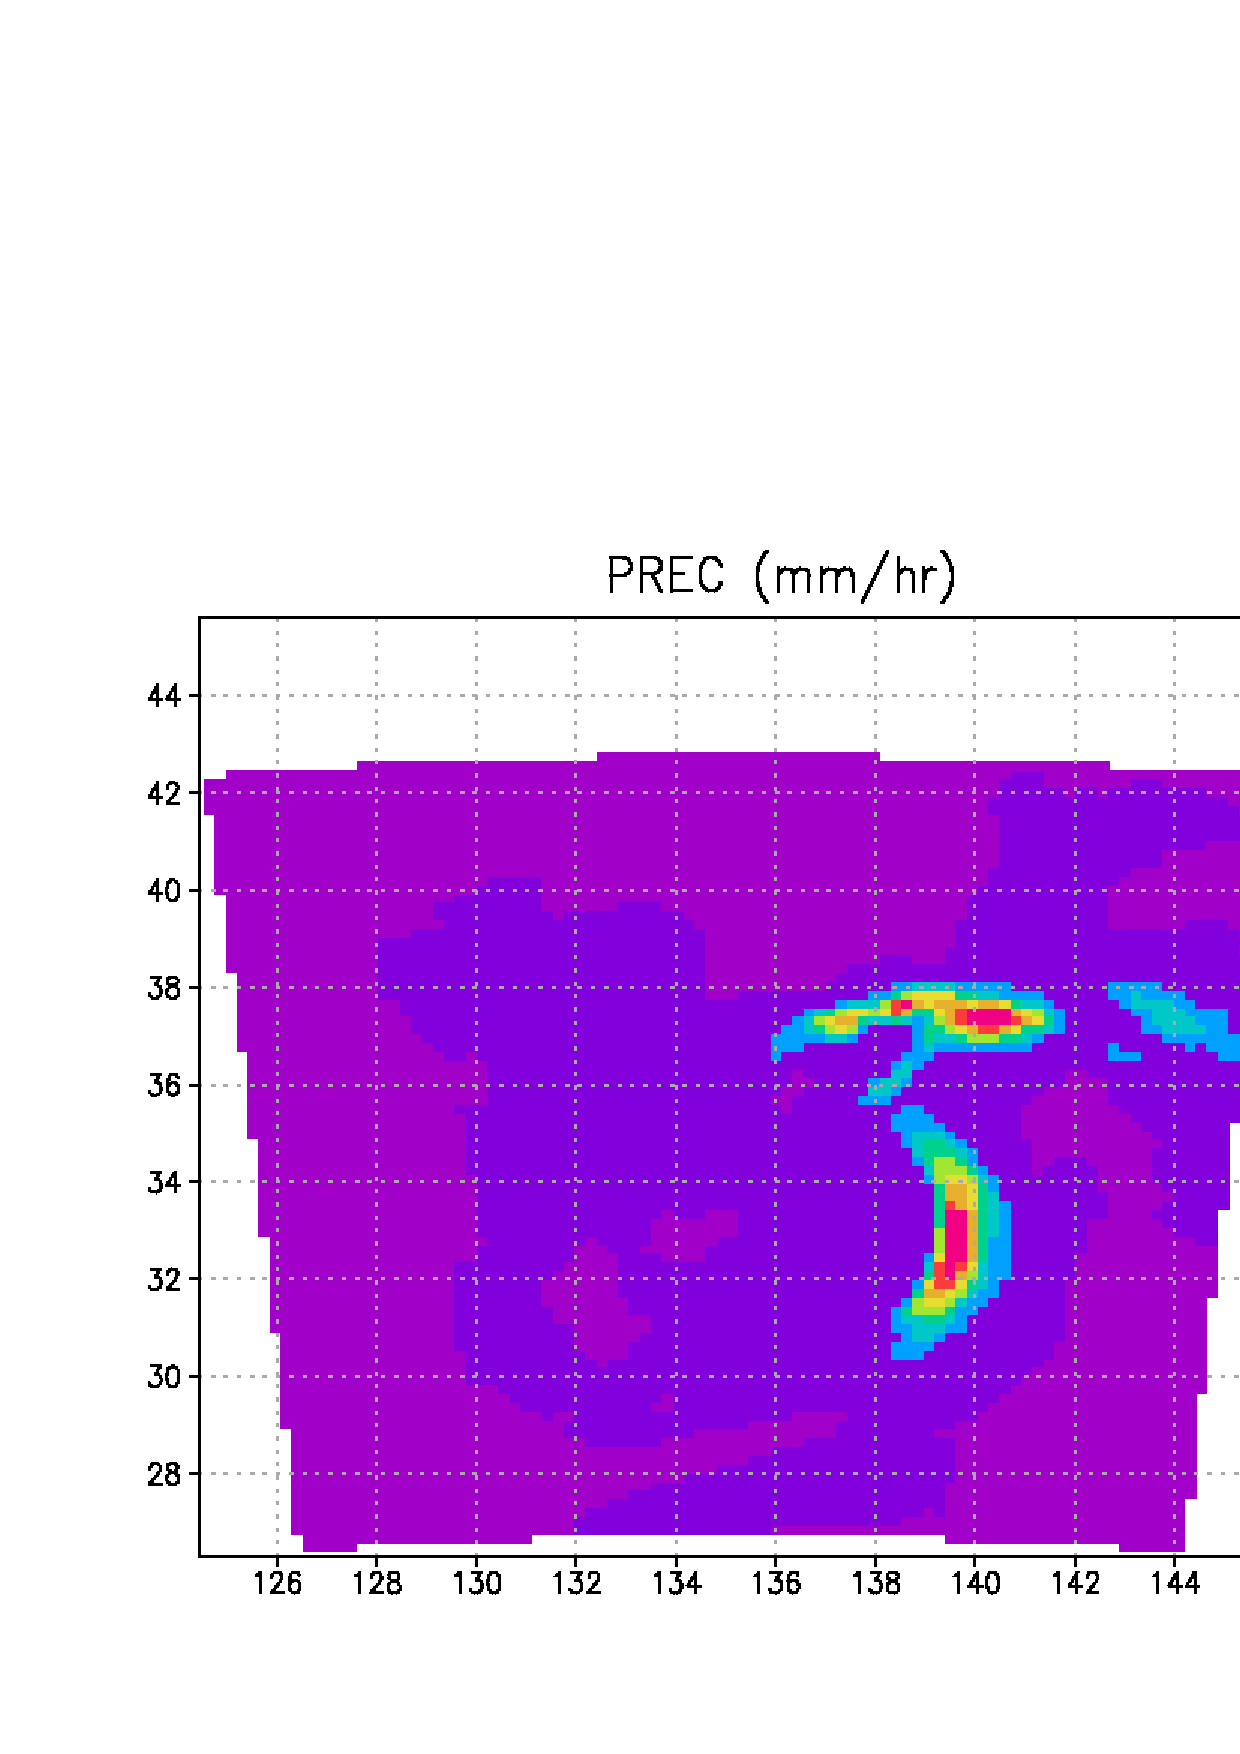
\includegraphics[width=0.55\hsize]{./../../figure/real_prec.pdf}\\
  \caption{計算開始から6時間後の降水フラックス}
  \label{fig:real_prec}
\end{center}
\begin{center}
  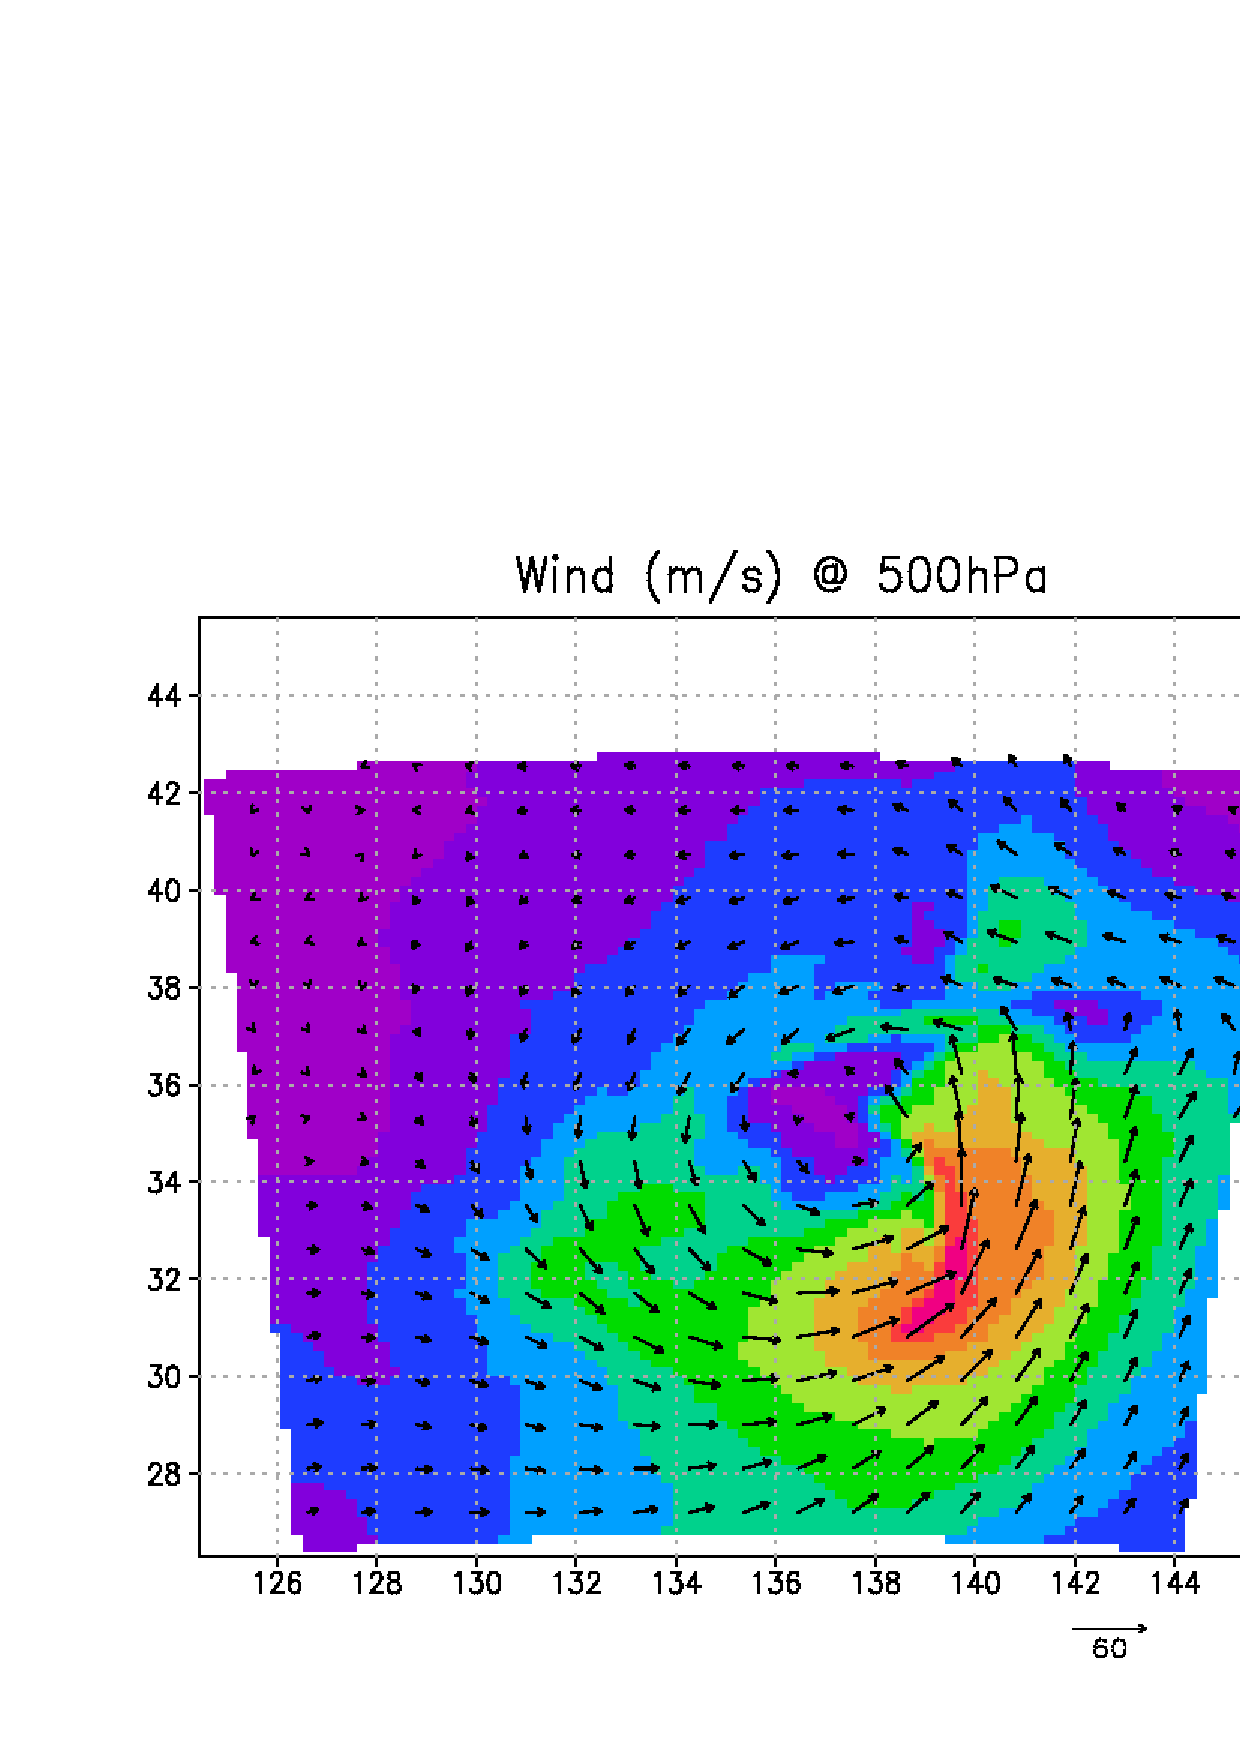
\includegraphics[width=0.55\hsize]{./../../figure/real_wind.pdf}\\
  \caption{計算開始から6時間後の850hPaの風速(色は絶対値、ベクトルは向き)}
  \label{fig:real_wind}
\end{center}
\end{figure}
